Having shown the potential that a DMP has to offer, this section now presents a simple scheme that is used to exploit the large energy savings available.
The main idea is to monitor at runtime some performance counters and make a decision at a regular interval on how to reconfigure the cores.
For this purpose, a model is trained offline using the data collected and presented earlier in the paper.
Once trained, the model predicts the optimal number of cores based on the performance counters from the previous time interval and reconfiguration occurs if it is different from the current number of cores.

\begin{figure}[t]
    \centering
	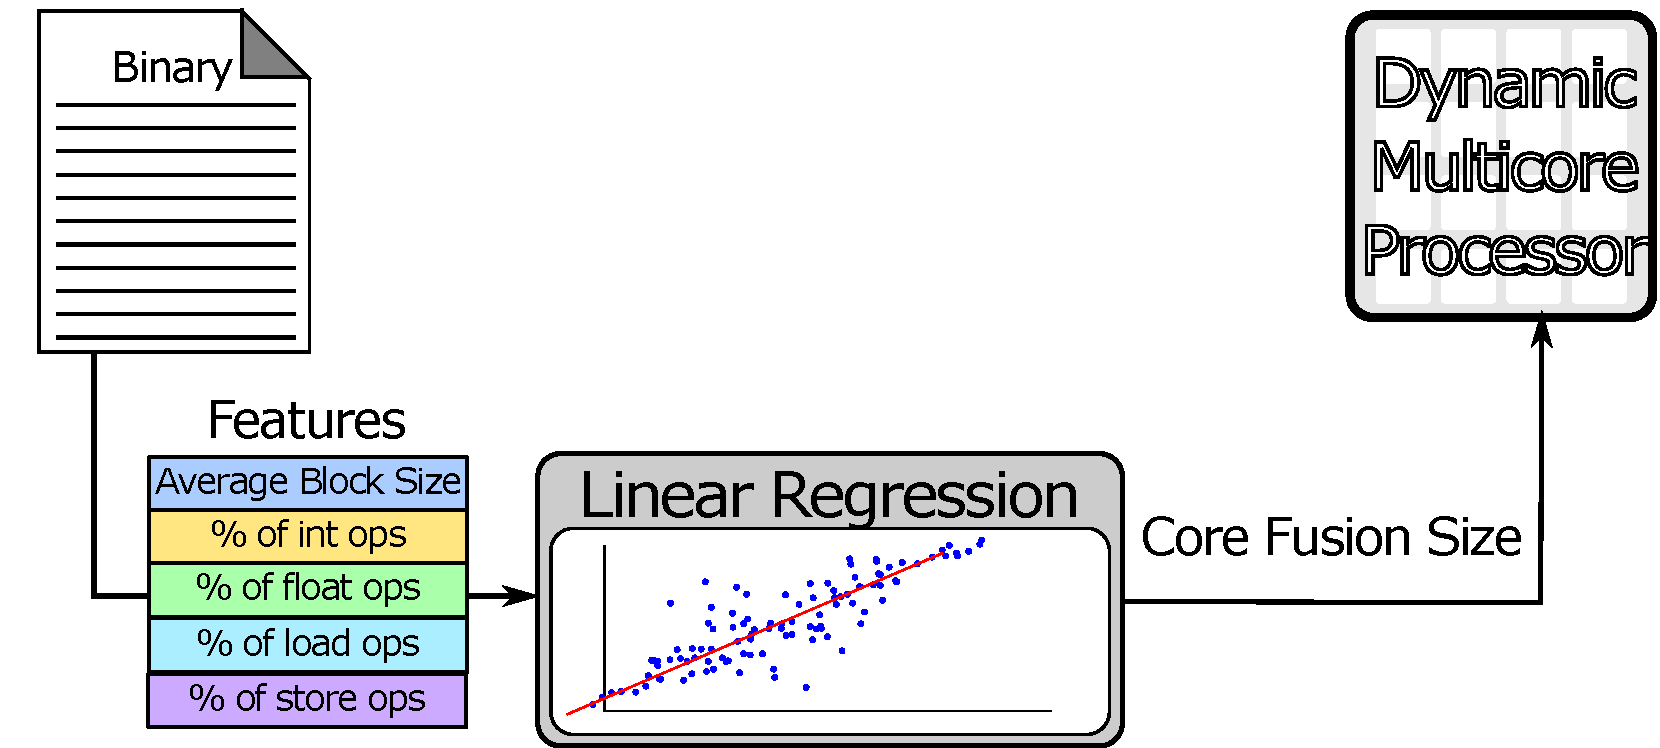
\includegraphics[width=0.7\textwidth]{cases-paper/graphics/other/model2.pdf}
    \caption{Linear Model.}
    \label{fig:linmod}
\end{figure}

\subsection{Model}

The model is linear regressor which makes predictions using a simple weighted sum of the input features, which is very lightweight and easy to integrate in hardware.
The model is trained offline using the traces gathered from the prior analysis for the \textbf{DSpeed} scenario which maximizes energy savings while maintaining performance.
Figure~\ref{linmod} is a graphical representation of the linear model used in this chapter.
The dataset consists of a set of four input features (average block size, and percentage of integer, floating point and load operations) and the optimal number of cores for each time tick for each program.
These features were chosen as they are easy to extract from the hardware.
To speedup the learning process, a single data point is created per phase, averaging the features of all the ticks in a phase, resulting in a total of 34 pairs of optimal core number and features.

The training consists of finding the weights that minimize the error when predicting the optimal number of cores to use across all time ticks and benchmarks.
Since only core configurations which use a power of two number of cores are considered, the linear model is built to predict the logarithm (base 2) of the number of cores.
The prediction is rounded up to the nearest integer in the interval $[0,4]$.
The following equation represents the trained linear model which can be used to make prediction:

\begin{align*}
  log_2(\textbf{\#cores}) = & -7.7\ +\ 0.028 \cdot \textbf{avgBlkSze}\ +\ 0.075 \cdot \textbf{\%int\_ops}\ +\\
 &0.069 \cdot \textbf{\%fp\_ops}\ +\ 0.21 \cdot \textbf{\%ld\_ops}
\end{align*}

For instance, if at runtime an average block size of 6 instructions, and 77\%, 1\% and 18\% of integer, floating point and load operations, respectively, then the predicted value will be 2.092.
Rounded up to the nearest integer value, 2, the optimal number of cores predicted will, therefore, be 4.

As can be seen, the largest weight is on the percentage of loads operations.
This is due to different reasons, mainly execution time and the fact that Load-Store Queues are fused.
When it comes to execution time, loads may take from 3 to 128 cycles depending on whether or not it is a cache miss or hit.
Whether it is a cache hit or miss, a block that takes longer to execute will often minimize the \textit{SynchronizationCost} penalty.
A block composed mainly of integer or floating point operations will often result in shorter execution rates; thus may execute faster, making it harder for large logical cores to improve performance.
More discussion on how the time it takes to execute a block influences the performance of LCs is discussed in Chapter~\ref{chp3}.
The other reason loads are prefered is due to the fact that loads can be fired independently to the Load-Store Queue.
Unlike stores that depend on previous memory instructions blocks being committed, loads can be fired with less overhead.
As data can be speculatively fetched, loads instructions can receive data from other cores before the data is stored, speeding up the load instruction.
By increasing the core count on load heavy blocks this will improve performance more reliably due to cores being able to issue loads in parallel.

\begin{figure}[t]
    \centering
	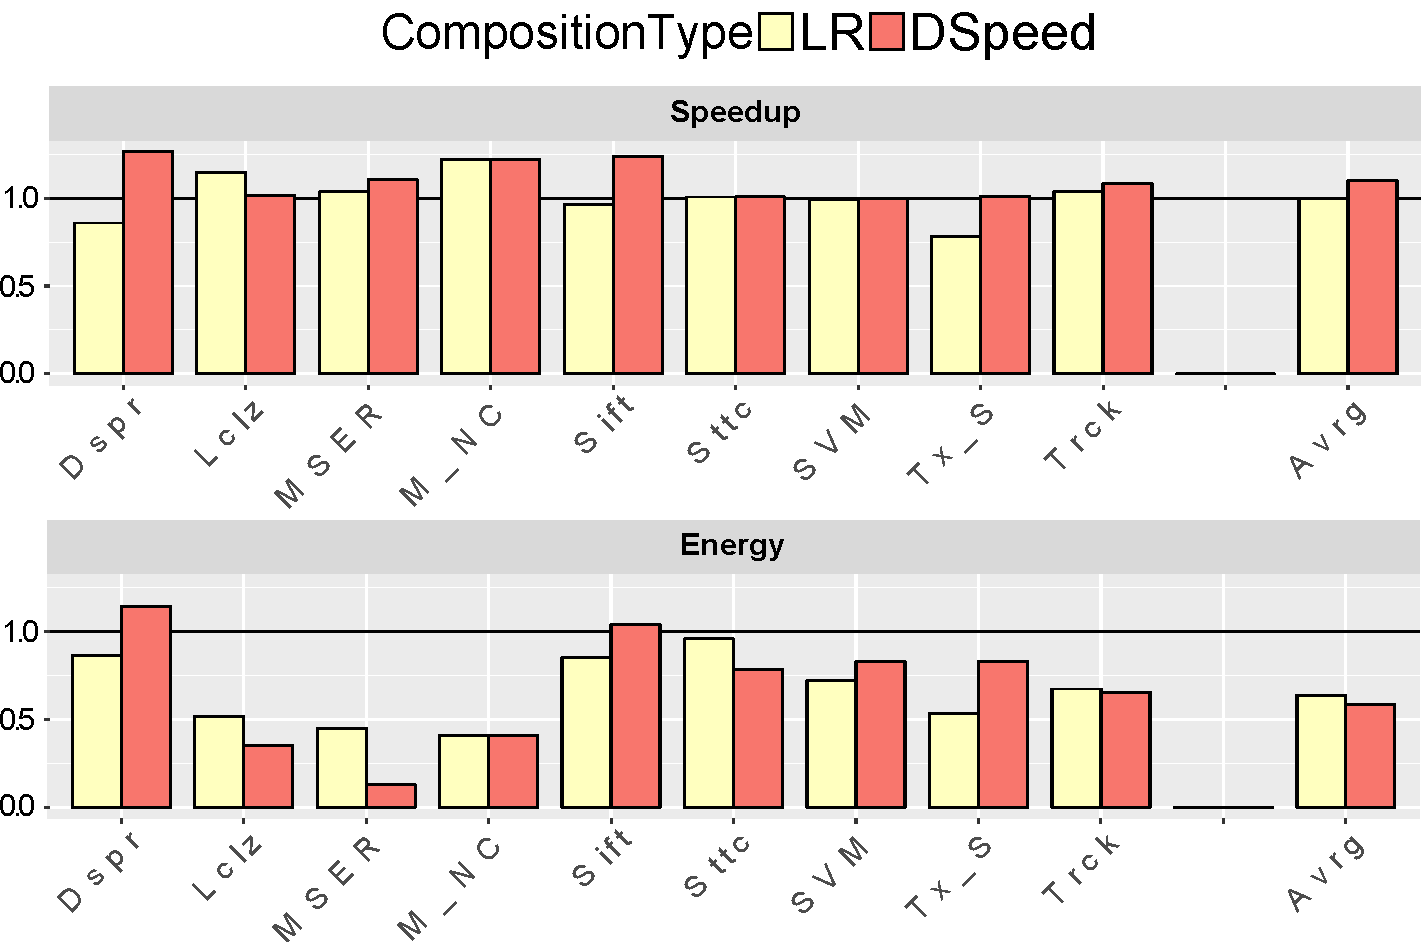
\includegraphics[width=1\textwidth]{cases-paper/graphics/results/lr_speed2.pdf}
    \caption{Performance results for maximizing speed for the SD-VBS benchmarks using the linear regressor (LR) model.}% For Speedup, higher means better, for energy lower is better.}
    \label{fig:speedlr}
\end{figure}

\subsection{Results}

To evaluate the performance of the model leave-one-out cross-validation  is used; it is a standard machine-learning methodology which tests the model using not seen during training.
For instance, if the model is tested for one program, let say \textit{Disparity}, the model is then trained using the dataset from all the other programs combined.
Then the resulting trained linear model is used to predict the optimal core number for each time tick of the disparity program and report the performance achieved.

Figure~\ref{fig:speedlr} shows the performance in terms of speed and energy that is achieved using the linear model normalized by a fixed static configuration.
The fixed configuration maximized performance across all the benchmarks using 8 cores and is the same as in the previous results presented in figure~\ref{fig:speedres}.
On average, the linear regressor model is able to consume 37\% less energy compared to the 8 cores fixed configuration and is able to exactly match its speed.

The performance is also compared with the best possible choice of dynamic reconfiguration, \textbf{DSpeed} which acts as an Oracle.
As can be seen, the linear model is able to exploit similar energy savings to the \textbf{Dspeed} scheme in most cases.
On average it reduces energy by 37\%, which is within 5\% of the 42\% achievable by the \textbf{Dspeed} scheme.
These results show that it is possible to implement a simple realistic lightweight scheme which offers large energy savings.
